\documentclass{tufte-handout}
%------------------------------------------------
%\geometry{showframe} % display margins for debugging page layout
%------------------------------------------------
\usepackage{graphicx} % allow embedded images
  \setkeys{Gin}{width=\linewidth,totalheight=\textheight,keepaspectratio}
  \graphicspath{{/home/swl/Dropbox/ucd/eu_economics/figs/}}  % set of paths to search for images
\usepackage{amsmath}  % extended mathematics
\usepackage{booktabs} % book-quality tables
\usepackage{units}    % non-stacked fractions and better unit spacing
\usepackage{multicol} % multiple column layout facilities
\usepackage{lipsum}   % filler text
\usepackage{fancyvrb} % extended verbatim environments
  \fvset{fontsize=\normalsize}% default font size for fancy-verbatim environments

%------------------------------------------------
% Standardize command font styles and environments
\newcommand{\doccmd}[1]{\texttt{\textbackslash#1}}% command name -- adds backslash automatically
\newcommand{\docopt}[1]{\ensuremath{\langle}\textrm{\textit{#1}}\ensuremath{\rangle}}% optional command argument
\newcommand{\docarg}[1]{\textrm{\textit{#1}}}% (required) command argument
\newcommand{\docenv}[1]{\textsf{#1}}% environment name
\newcommand{\docpkg}[1]{\texttt{#1}}% package name
\newcommand{\doccls}[1]{\texttt{#1}}% document class name
\newcommand{\docclsopt}[1]{\texttt{#1}}% document class option name
\newenvironment{docspec}{\begin{quote}\noindent}{\end{quote}}% command specification environment
%------------------------------------------------

%------------------------------------------------
%%%% Details %%%%
%------------------------------------------------
\title{European Economy: Economic growth}
\author{University College Dublin}
\date{Spring 2017} 
\begin{document}
\maketitle  
%------------------------------------------------------------------------------
% MACROECONOMIC INTEGRATIONS
\section{Macroeconomic integration}
Before we dive into examining economic growth in the European Union, first a short recap of the different stages of macroeconomic integration.\footnote{We will discuss further integration at the end of this lecture and in the next lecture as well.}
Balassa identified 6 different stages
\begin{enumerate}
  \item Preferential customs area
  \item Free trade area
  \item Customs union
  \item Common market
  \item Economic and monetary union
  \item Political union
\end{enumerate}
Over time the European community has progressed through various of these stages and with the creation of the European Union they are now roughly in between stage 5 and 6. 
Now in a lot of areas there is movement towards further integration to form a political union, but among various member states there is some friction concerning whether this is a desirable step. 
Certainly the Eurocrisis and the recovery from it has illustrated that large economic differences still exist across the member states and it has also highlighted the difficulties the EU has in solving a crisis of this magnitude.\footnote{This equally applies to the refugee crisis.}
One could argue that certain challenges that Europe faces are best dealt with by a larger political union, such as policy related to defence or climate change. Other policy issues, such as pension funds or drugs legalisation, are possible better left to the devices of the individual member states.
Let's consider the ways through European integration actually might contribute to economic growth. 
Recall that the original purpose of European integration, besides ensuring political stability, was to achieve steady economic growth rates providing higher living standards.\footnote{In terms of political stability, by making the economic welfare of Germany and France dependent on each other, war would be extremely costly.} 
\clearpage

Some ways in which economic growth can be affected is through
\begin{enumerate}
  \item International factors
  \begin{itemize}
    \item Exchange rate regimes
    \item Terms of trade
    \item Capital flows
  \end{itemize}

  \item Setting policy\footnote{We will return to this topic later.}
  \begin{itemize}
    \item Promoting competitiveness and growth
    \item Encouraging full employment and improve quality of work
    \item Social protection and cohesion
  \end{itemize}  
\end{enumerate}

%------------------------------------------------------------------------------
% GROWTH ACCOUNTING
\section{Growth accounting}
How do we measure growth and the factors that contribute to growth? 
Suppose that we model total economic output using the following Cobb-Douglas production function
\begin{align*}
  Y_t=A_tK^{\alpha}_tL^{\beta}_t
\end{align*}

Where $K$ is capital, $L$ labour, and $A$ accounts for technology. 
Technology is an important factor in explaining economic growth for the following reasons
\begin{itemize}
  \item Increase in $A_t$ results in higher output without having to raise inputs
  \item Measure of productive efficiency
  \begin{itemize} 
    \item Can fluctuate for various reasons, e.g. new technology, government regulation, management style
  \end{itemize}
\end{itemize}

Since an increase in $A_t$ increases productiveness of other factors, it is also known as Total Factor Productivity (TFP).
Analysing economic performance across countries we are often interested in productivity or output per worker, which in our model is given by
\begin{align*}
  \frac{Y_t}{L_t}= A_t \left(\frac{K_t}{L_t} \right)^{\alpha}L_t^{\alpha + \beta -1}
\end{align*}

This function shows that there are potentially three ways to increase productivity
\begin{enumerate}
  \item Increase the number of workers
  \begin{itemize}
    \item Will add to growth if $\alpha+\beta>1$
    \item Most growth theories assume constant returns to scale\footnote{$\beta=1-\alpha$} so the production functions becomes
    \begin{align*}
      \frac{Y_t}{L_t}= A_t \left(\frac{K_t}{L_t} \right)^{\alpha}
    \end{align*}
  \end{itemize}
  \item Capital deepening\footnote{i.e. increasing the amount of capital per worker}
  \item Technological progress  
\end{enumerate}

%------------------------------------------------------------------------------
% SWAN-SOLOW MODEL
\subsection{Swan-Solow model}
In the standard Swan-Solow model the production functions links output to capital and labour inputs as well as a technological efficiency parameter.
\begin{align*}
  Y_t = AF(K_t,L_t) 
\end{align*}


A key feature of the model is that, with a constant labour supply, there are diminishing marginal returns to capital accumulation meaning that each increase in capital will give a progressively smaller increase in output\footnote{
\begin{align*}
  \frac{\delta^2Y_t}{\delta K_t}<0
\end{align*}}

Additional assumptions of the model include that it is a closed economy, with no government sector or international trade. 
This means that all output takes the form of either consumption or investment, where savings will equal investments
\begin{align*}
      Y_t &= C_t+I_t\\
      S_t &= Y_t-C_t=I_t
\end{align*}
 
Importantly, capital depreciates and therefore the capital stock will depend positively on investments and negative on the depreciation rate $\delta$.
\begin{align*}
  \frac{dK_t}{dt}=I_t -\delta K_t
\end{align*}

The model makes no assumptions about consumption preferences, so consumers will save a constant share of income. 
Which entails that investments will also be a constant fraction of output
\begin{align*}
  S_t = sY_t = I_t
\end{align*}

This means that the level of investments is given by
\begin{align*}
  I_t=sY_t=sAF(K_t,L_t)
\end{align*}
which means that a one off increase in technology level $A$ has the same effect as a one off increase in $s$: capital and output gradually increase to a new level.
Nonetheless, the model implies a very important difference between these two determinants of growth.
Note that the savings rate $s$ is subject to a limit, whereas as $A$ does not face such constraints. 
Therefore, in order to have long-term sustainable growth increases in TFP matter.\footnote{Specifically, growth through capital accumulation will taper off over time producing a one-off increase in output per worker whereas TFP growth can lead to sustained higher growth rates of output per worker.} 

%------------------------------------------------------------------------------
% GROWTH IN THE EU
\section{Economic growth in Europe over time}
Despite the hegemony of European countries in the world from about 1500 onward, the situation on the continent looked pretty bleak in the aftermath of the Second World War which brought a lot of destruction. 
However, thanks to large public investments, some financial aid from the US\footnote{The Marshall Plan}, and closer economic ties following the Treaty of Rome, the European countries actually experienced relatively high growth rates in the second half of the twentieth century and the establishment of the welfare state. 
At least in Western Europe, as countries in the East adopted communism becoming de facto Soviet satellite states.\footnote{The strong economic performance of (West) Germany and Italy, two members of the G8, are particularly impressive given that they were Axis powers.}
Two analyse economic growth in Europe we will take two approaches
\begin{enumerate}
  \item Compare it to the US
  \item Track development of new EU member states
\end{enumerate}

%------------------------------------------------
% FIGURE: 
\begin{figure} \centering
    \includegraphics[scale=.3]{growth_difference}
    \includegraphics[scale=.3]{gdp_per_capita}
    \caption{Difference GDP growth of the EU-15 with the USA (top) and GDP per capita over time, solid black line is USA (bottom). Data: World Bank World Development Indicators}
    \label{fig:growth}
  \end{figure}
%------------------------------------------------

The upper panel of figure~\ref{fig:growth} shows the difference of the EU-15 compared to the USA, and illustrates that there have been periods were growth in the EU was larger than in the USA. 
The increase in GDP from the 1950s till the mid-1990s was spurred by a strong growth in labour productivity in the Western European countries.
However, since the mid-1990s labour productivity in the USA has started to grow faster again. 
Indeed, figure~\ref{fig:comparison} illustrates that compared to GDP per capita levels in 1980 few European countries have grown faster than the US.
\newline
%------------------------------------------------
% FIGURE: 
\begin{figure} \centering
    \includegraphics[scale=.3]{comparison_us}    
    \caption{Comparing economies of the EU15 with the US. Data: World Bank World Development Indicators}
    \label{fig:comparison}
  \end{figure}
%------------------------------------------------
From an American perspective the slowdown or reduction in Europe's productivity can be attributed to a number of growth impeding factors including
\begin{enumerate}
  \item Taxation level
  \item Regulations
  \item Level of competition
\end{enumerate}

Arguably the US is doing a better job in allocating capital and labour and also has higher TFP level. 
However, one must bear in mind that in the US income equality is higher and it doesn't provide the same level of social security as many European states do.
Probably the best period in post-war European growth was between 1950-1973. 
This period covers the the recovery from the war, which saw a lot of public money spent on investments and the shift from labour from the agricultural sector to other sectors of the economy, up until the oil price crisis. 
One factor contributing to growth during this period is the opening up of markets thanks to European integration.\footnote{Recall that the common market was established in 1957 by the Treaty of Rome.}
%--------------------------------------
\begin{figure}
  \includegraphics[scale=.3]{unit_labour_costs}
  \label{fig:ulc}
  \caption{Unit labour costs, 1999=100. The red line indicates Spain, yellow Germany, and the dashed black line the Eurozone average of the 12 original member states. The diagonal black line is a 2\% inflation target.}
\end{figure}
%--------------------------------------
Despite early success, growth has slowed down in Europe and lack of competitiveness has regularly been identified as one of the culprits. 
Although competitiveness is difficult to measure, an often used proxy is relative unit labour costs, or the labour compensation costs, including taxes and social security, per unit of output. 
These costs will increase when the growth rate of the nominal wages out paces labour productivity. 
Since labour costs are an important determinant of prices, policy makers in the eurozone prefer the growth in costs to be under the inflation target of 2 percent. 
Figure~\ref{fig:ulc} shows the development of labour costs for the original 12 eurozone countries and illustrates that only a few have been able to keep costs below the targeted inflation rate. 
The crisis has severely affected wage setting particularly in Greece and Ireland. 

%--------------------------------------
\begin{figure}
  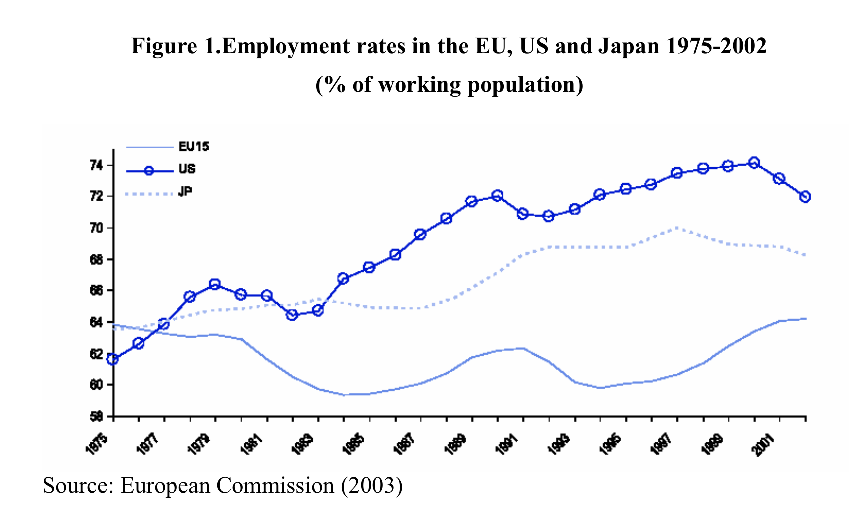
\includegraphics[scale=.3]{employment_rate}
  \label{fig:employment}
  \caption{Employment rate in the EU compared to the US and Japan. Figure taken from \href{http://www.eui.eu/Documents/RSCAS/Research/EFN/Reports/Annex2004Autumn/Annex5autumn2004.pdf}{"Annex 5: Supply-side reforms in Europe: Can the Lisbon Strategy be repaired? "}}
\end{figure}
%--------------------------------------


Another major issue in the EU is the employment rate (figure~\ref{fig:employment}).
EU GDP per capita is about 35\% below that of the US\footnote{This is for the EU28.} which is due to the fact that Europeans work less, as output-per-hour worked is comparable. 
Europeans work less because fewer of them are employed and generally two reasons for this are given
\begin{enumerate}
  \item Relatively few new jobs are created
  \item Unemployed Europeans spend more time searching for employment
\end{enumerate}

%------------------------------------------------------------------------------
% GROWTH NEW MEMBERS
\section{Growth after joining the EU}
So far we have only examined growth of European countries over time, comparing it to the USA. 
But we haven't really looked at the effect of the EU on economic growth for individual member states. 
Now estimation the effect of joining the EU on economic growth can be difficult, since it is hard to establish a counterfactual. 
Nonetheless, we can still examine the development of output growth over time since joining the union for a number of countries by doing a simple exploratory data analysis. 
Over the years there have been a number of enlargement rounds:
\begin{enumerate}
  \item During the 1970s Denmark, the United Kingdom, and Ireland joined
  \item In the 1980s there was the inclusion of former military regimes; Greece, Portugal, and Spain
  \item Joining of non-aligned countries after the end of the Cold War in 1995; Austria, Finland, and Sweden
  \item And during the 2000s a number of former East Bloc countries joined the EU. 
\end{enumerate} 

In general joining the EU has been thought of as being beneficial, although there is of course cross-country variation.\footnote{An exception might be Greece.} 
The next set of figures (figure~\ref{fig:enlargement1},~\ref{fig:enlargement2},~\ref{fig:enlargement3},~\ref{fig:enlargement4}) shows GDP over time for a selection of countries in each enlargement round. 
The GDP is standardised to compare to the average of the  Organisation for Economic Co-operation and Development (OECD), which is a group consisting of the richest countries in the world.\footnote{Note that the OECD has also had various enlargements over the years.}
In each figure the horizontal dotted line shows the country average before joining the EU, and the vertical dotted line is the year of membership. 
So for instance figure~\ref{fig:enlargement1} illustrates that Ireland has experienced very positive GDP growth over the past decades since joining the EU, compared to the OECD average.\footnote{Note that all GDP data is at Purchasing Power Parity to account for relative living standards across countries and time.} 
In contrast, for Denmark and Great Britain it seems that not much has actually changed. 
Indeed, both these countries find their GDP level to be slightly below the average before joining the EU, but in both cases the decreasing trend seems to have started before actually joining. 
%------------------------------------------------
% FIGURE: 
\begin{figure} \centering
    \includegraphics[scale=.3]{first_enlargement.png}
    \caption{Tracking development of GDP, relative to OECD average, over time for countries in the first wave of EU enlargement during the 1970s. New members included Denmark, Great Britain, and Ireland. Data: Penn World Tables}
    \label{fig:enlargement1}
  \end{figure}
%------------------------------------------------

For the Southern European countries (fig~\ref{fig:enlargement2}) the figure illustrates that the situation in Greece has deteriorated in the past years, while for Spain and Portugal there has been a positive upward trend since joining the EU. 
For the formerly non-aligned countries (fig~\ref{fig:enlargement3}) the figure again illustrates a very mixed pattern. 
For this group of countries it seems that the long term trend in GDP is somewhat independent of EU membership.
%------------------------------------------------
% FIGURE: 
\begin{figure} \centering
    \includegraphics[scale=.3]{second_enlargement.png}
    \caption{Tracking development of GDP, relative to OECD average, over time for countries in the first wave of EU enlargement during the 1980s. New members included the Southern European countries Greece, Portugal, and Spain after the end of military dictatorships. Data: Penn World Tables}
    \label{fig:enlargement2}
  \end{figure}
%------------------------------------------------
\clearpage
For the three countries that joined in 1995, an evaluation was made in 2005 to examine the impact of joining the EU 10 years later. 
In general this evaluation showed that joining the EU had been beneficial. 
\begin{itemize}
  \item Austria
  \begin{itemize}
    \item There is an associated welfare effect of 2\% the result of lower prices
    \item There is an additional 0.5\% GDP growth per year
  \end{itemize}
  \item Finland
  \begin{itemize}
    \item EU membership boosted trade and investment
    \item It lowered prices for consumers
    \item Joining the EMU had a bigger overall impact on the economy
  \end{itemize}
  \item Sweden
  \begin{itemize}
    \item There was an estimated 0.4\% increase in trend growth
    \item This increase was due to increased competition, a sharp increase in FDI and an improvement in fiscal and monetary policy\marginnote{Sweden experienced a severe banking crisis in 1991-92, very similar to what the USA experienced in 2007-08.}
  \end{itemize}
\end{itemize}
%------------------------------------------------
% FIGURE: 
\begin{figure} \centering
    \includegraphics[scale=.3]{third_enlargement.png}
    \caption{Tracking development of GDP, relative to OECD average, over time for countries in the first wave of EU enlargement during the 1990s. New members include Austria, Finland, and Sweden who were neutral during the Cold War. Data: Penn World Tables}
    \label{fig:enlargement3}
  \end{figure}
%------------------------------------------------
Finally, looking at some of the countries that recently joined, the data shows a upward trend. 
In this case we must be cautious drawing too strong conclusions since these countries just recently joined the EU, so we can't say anything thing about the effect on the long term. 
Moreover, the economic development that these countries are currently experiencing might be driven by the fact that they went from a planned economy to a more free market economy, with increased trade levels. 
%------------------------------------------------
% FIGURE: 
\begin{figure} \centering
    \includegraphics[scale=.3]{fourth_enlargement.png}
    \caption{Tracking development of GDP, relative to OECD average, over time for countries in the first wave of EU enlargement during the 2000s. New members include, amongst others, Czechia, Hungary, and Poland, former East Bloc countries. Data: Penn World Tables}
    \label{fig:enlargement4}
  \end{figure}
%------------------------------------------------
\clearpage
%------------------------------------------------------------------------------
\subsection{Example: Growth accounting in the Euro area}
As already mentioned, growth in Europe was very similar to that of the US. 
However, since the 1990s US GDP growth has been about 1.3 percentage points higher than that in Europe. 
Figure~\ref{fig:euro} shows growth accounting calculations for the euro area over time and illustrates that output per worker has declined over time, specifically TFP growth.
One worrying aspect is that the composition of past growth shows that output growth has mainly relied on increases in capital and labour input, and not so much on improvements in total factor productivity. 
This is troublesome since the Swan-Solow model highlights that capital is endogenous and depends on technological efficiency. 
%--------------------------------------
\begin{figure}
  \includegraphics[scale=.3]{mcquinn_whelan}
  \includegraphics[scale=.3]{mcquinn_whelan2}
  \label{fig:euro}
  \caption{Growth accounting in the Eurozone. Based on work by McQuinn and Whelan \href{http://www.karlwhelan.com/Papers/McQuinnWhelanMarch2015.pdf}{Europe's Long-Term Growth Prospects: With and Without Structural Reforms}.}
\end{figure}
%--------------------------------------

Besides the slump in TFP, one other serious issue that is affecting Europe's potential growth is the aging pattern. 
Population growth in Europe is slowing down and expected to peak in the middle of the century (figure~\ref{fig:population}).
More worryingly, the population aged between 15-64 years, those that make up the working population, has peaked already and is set to decline. 
This trend likely leads to a further reduction in the number of hours worked, assuming that the employment rate returns to pre-crisis levels, which again likely reduces output growth.
%--------------------------------------
\begin{figure}
  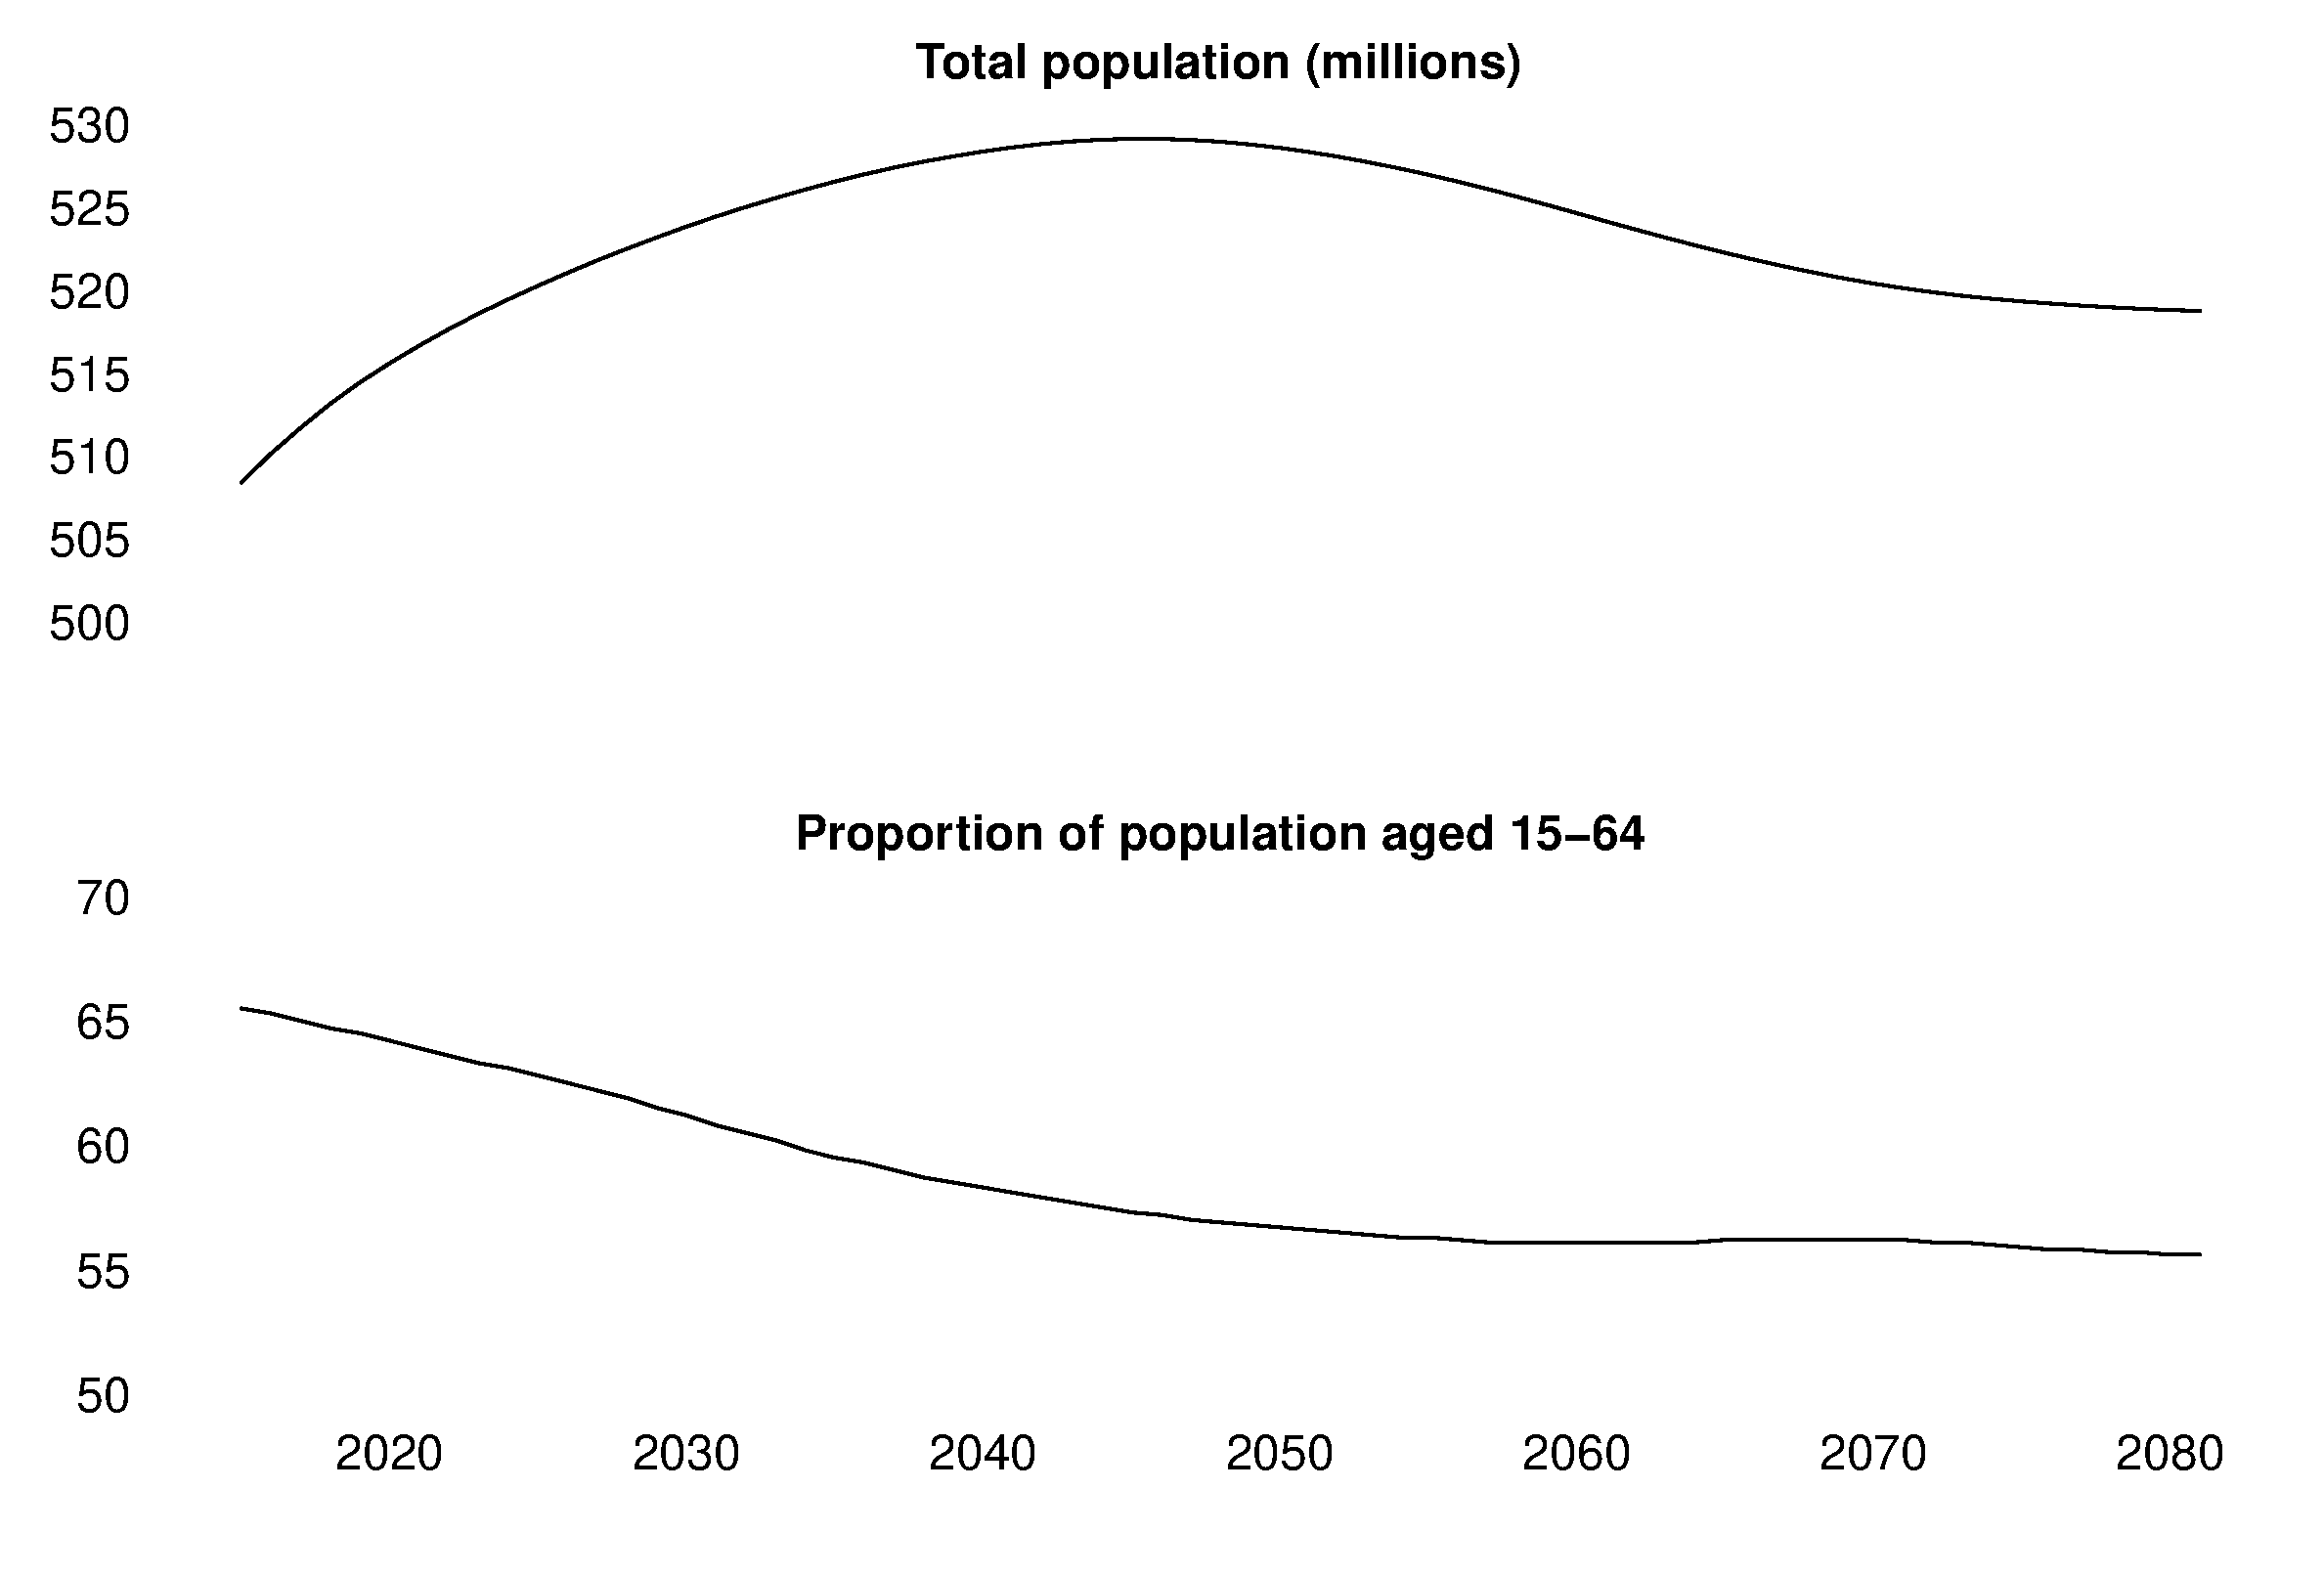
\includegraphics[scale=.3]{population}
  \label{fig:population}
  \caption{Demographic projections for the European Union (28). Data: Eurostat}
\end{figure}
%--------------------------------------
\newline
The macroeconomic problems that Europe faces are twofold
\begin{enumerate}
  \item Short term
  \begin{itemize}
    \item Weak aggregate demand
    \item High levels of public and private debt
  \end{itemize}
  \item Long term
  \begin{itemize}
    \item Demographic challenges  
  \end{itemize}    
\end{enumerate}



%------------------------------------------------------------------------------
% POLICY
\section{Policies to promote growth}
In order to boost productivity and labour market participation, the EU countries could implement structural reforms which include areas such\footnote{Based on McQuinn \& Whelan (2015), \href{http://www.karlwhelan.com/Papers/McQuinnWhelanMarch2015.pdf}{Europe's Long-Term Growth Prospects: With and Without Structural Reforms}.} 
\begin{enumerate}
  \item Labour market
  \begin{itemize}
    \item Aims at reducing long-run unemployment rates
    \item e.g. protection against dismissals, regulation of part-time work
  \end{itemize}
  \item Pension
  \begin{itemize}
    \item Workers can work to a later age
    \item Similar to Switzerland where there is a relatively high rate of labour participation among older workers
  \end{itemize}
  \item Broader regulatory reforms
  \begin{itemize}
    \item e.g. taxes, education policies, etc. 
  \end{itemize}
\end{enumerate}


A first attempt by the EU to collectively address Europe's productivity problems was the 2000 Lisbon Strategy.
This strategy aimed at improving the state of the European economy by turning the EU into "the most dynamic, knowledge based economy in the world by 2010".\footnote{At the time the EU was behind the US in most technical and scientific fields which poses problems for future economic growth.} 
The Lisbon strategy focused mainly on deregulation of the labour and product markets.
Some of the impediments to growth identified by the Lisbon Declaration included\footnote{Taken from \href{http://voxeu.org/article/failure-lisbon-strategy}{"The failure of the Lisbon strategy"}}
\begin{itemize}
  \item Problems posed by the public sector
  \begin{itemize}
    \item Risk-taking was discouraged by large bureaucracies
    \item Public services that are often inefficient
    \item Policies that protect jobs rather than people
  \end{itemize}
  \item The salience of national interests
  \begin{itemize}
    \item Protectionist measures that inhibit competition in the services sector
    \item Absence of unified research space
  \end{itemize}
\end{itemize}

To achieve the strategy's objective, the policy implemented supply-side reform using what was called the Open Method of Coordination (OMC).
This method meant that there was no need for a centralised approach from Brussels, but nonetheless the national governments were required to take more action in implementing structural reforms. 
The Lisbon Strategy set out to take the following actions\footnote{Taken from \href{http://cordis.europa.eu/programme/rcn/843_en.html}{"The Lisbon Strategy for growth and jobs"}}
\begin{itemize}
  \item Investing more in young people, education, research and innovation to generate wealth and provide security for every citizen
  \item Opening up markets
  \item Cutting red tape
  \item Investing in modern infrastructure to help enterprises grow, innovate and create jobs
  \item Developing a skilled entrepreneurial workforce
  \item Ensuring a society with high levels of employment, social protection and a healthy environment
\end{itemize}

Despite good intentions the Lisbon Strategy failed mainly through lack of political will. 
In 2010 a new 10-year strategy was rolled out called \href{http://ec.europa.eu/europe2020/europe-2020-in-a-nutshell/index_en.htm}{Europe 2020}. 
The strategy identified that the responsibility for structural reforms lies with the national governments but that they should rely on the European single market and the common trade policy. 
The strategy focuses on a number of key issues
\begin{enumerate}
  \item Employment
  \begin{itemize}
    \item Target of 75\% employment rate of 20-64-year-olds
  \end{itemize}
  \item Innovation
  \begin{itemize}
    \item Invest 3\% of EU's GDP in R\&D
  \end{itemize}
  \item Climate/energy
  \begin{itemize}
    \item Limit greenhouse gasses by 20-30\% compared to 1990 levels
    \item 20\% of energy requirements coming from renewable energy
    \item Increasing energy efficiency by 20\%
  \end{itemize}
  \item Education
  \begin{itemize}
    \item Reduce school dropout rate below 10\%
    \item 40\% of 30-34 years old completing tertiary education
  \end{itemize}
  \item Social inclusion
  \begin{itemize}  
    \item Reduce people at risk of poverty or social exclusion with 20 million
  \end{itemize}
\end{enumerate}


%------------------------------------------------------------------------------
\section{Further integration: Adopting the Euro}
In 2004 the EU-15 was expanded by 10 countries, 8 of which were former communist states.\footnote{The other two being Cyprus and Malta.}
Currently, of those 10 new member states, 7 have joined the Eurozone whereas Czechia (formerly Czech Republic), Hungary, and Poland still hold their own currency. 
Given the recent crisis one could wonder whether it made sense for some of these countries to join the euro, and whether it is beneficial for the Eurozone itself. 
From the perspective of optimal currency area theory it would make sense for these countries to join given that they
\begin{itemize}
  \item are relatively small economies
  \item very open in terms of trade
  \item vulnerable to speculative attacks on their currency
\end{itemize}

Figure~\ref{fig:new_members} illustrates the size of the economies of the new member states, relative to that of Germany, versus the openness of trade. 
The openness of trade, measured in ratio to GDP, ranges from 70 to 130\%. 
This is actually still relatively low given for instance their economic size and distance to trading partners.
Small open economies such as those from Central Europe are vulnerable to speculative attacks on their currency. 
The daily global turnover in the global foreign exchange market can reach \textdollar4 to 5 trillion. 
A large hedge fund might have access to more resources than the monetary authority of most new member states, implying that a national currency can become a liability.
%------------------------------------------------
% FIGURE: 
\begin{figure} \centering
    \includegraphics[scale=.3]{new_member_states.png}
    \caption{Economic size and openness of new EU member states joined in 2000s. Red line indicates Portugal. Data: World Bank}
    \label{fig:new_members}
  \end{figure}
%------------------------------------------------

One argument against these countries joining the Eurozone is that they are too poor. 
However this gap is closing and some countries have already overtaken Portugal (figure~\ref{fig:gdp_per_capita}). 
The obvious cost to the countries joining the euro is that they have to give up autonomy over monetary policy, which can't be used any more to stabilise country-specific shocks.\footnote{Note that implementing monetary policy for stabilisation is hard since shocks are hard to identify and monetary policy itself is subject to lags which are often long and variable.} 
Interestingly, in contrast with some of the more senior member states, labour mobility is much higher between the Central European member states and some of the EU members that didn't impose immigration restrictions. 
As such, labour mobility can help address country-specific shocks.\footnote{However, this relatively high degree of labour mobility arguably also contributed to Brexit.}


%------------------------------------------------
% FIGURE: 
\begin{figure} \centering
    \includegraphics[scale=.3]{gdp_per_capita2}
    \caption{GDP per capita in 2015 where EU-28=100. Data: Eurostat}
    \label{fig:gdp_per_capita}
  \end{figure}
%------------------------------------------------


%------------------------------------------------------------------------------
\end{document}
